\chapter{加性模型、树及相关方法}

第 9 章开始讨论监督学习的若干具体方法。这些方法都对未知回归函数假设某种（不同的）结构化形式，从而缓解\textbf{维数灾难}；代价是可能误设模型，因此每处都需要权衡。本章介绍五种相关技术：\textbf{广义加性模型（GAM）、树（trees）、多元自适应回归样条（MARS）、患者规则归纳法（PRIM）与专家分层混合（HME）}。本节先介绍其中的广义加性模型。

% ============ §9.1 广义加性模型 ============
\section{广义加性模型}

传统线性模型虽然简洁，但现实效应往往非线性。此前章节用预定义基函数实现非线性；本节介绍更自动、灵活的统计方法——\textbf{广义加性模型（Generalized Additive Models, GAM）}，用于识别和刻画非线性回归效应。

\subsection{模型定义}

回归设置下，广义加性模型形式为
\begin{equation}\label{eq:9_1}
    \E(Y \mid X_1, X_2, \ldots, X_p) = \alpha + f_1(X_1) + f_2(X_2) + \cdots + f_p(X_p)
\end{equation}
其中 $f_j$ 是未指定的光滑（非参数）函数。与第 5 章「每个函数用基函数展开」不同，这里用\textbf{散点图平滑器}（如三次平滑样条或核平滑器）拟合每个函数，并提供同时估计全部 $p$ 个函数的算法（§9.1.1）。

二分类情形（logistic）：回忆 §4.4 的二元数据 logistic 回归，把响应均值 $\mu(X) = \Pr(Y=1 \mid X)$ 通过 logit 链接与预测变量线性相连。加性 logistic 回归把每个线性项换成更一般的函数形式：
\begin{equation}\label{eq:9_3}
    \log\frac{\mu(X)}{1-\mu(X)} = \alpha + f_1(X_1) + \cdots + f_p(X_p)
\end{equation}
非参数形式使模型更灵活，但\textbf{保留可加性}，因此解释方式与线性模型类似。加性 logistic 回归是 GAM 的一个例子。

一般地，响应 $Y$ 的条件均值 $\mu(X)$ 通过\textbf{链接函数} $g$ 与预测变量的加性函数相连：
\begin{equation}\label{eq:9_4}
    g[\mu(X)] = \alpha + f_1(X_1) + \cdots + f_p(X_p)
\end{equation}

\textbf{常见链接函数：}
\begin{itemize}
    \item $g(\mu) = \mu$：恒等链接，用于高斯响应数据的线性/加性模型
    \item $g(\mu) = \mathrm{logit}(\mu)$ 或 $g(\mu) = \mathrm{probit}(\mu) = \Phi^{-1}(\mu)$：二项概率
    \item $g(\mu) = \log(\mu)$：Poisson 计数数据的对数线性/对数加性模型
\end{itemize}
这三类都来自指数族抽样模型（还包括 gamma、负二项分布），构成著名的\textbf{广义线性模型（GLM）}，并同样推广为广义加性模型。

\textbf{GAM 的灵活性：}
\begin{itemize}
    \item 可混合线性与非线性项——当某些输入是定性变量（因子）时需要参数形式
    \item 非线性项不限于主效应：可以是两个以上变量的非线性分量，或对因子 $X_k$ 每个水平给出独立曲线
    \item 例：$g(\mu) = X^T\beta + \alpha_k + f(Z)$（半参数模型，$X$ 线性建模、$Z$ 非参数、$\alpha_k$ 是定性输入 $V$ 第 $k$ 水平效应）；$g(\mu) = f(X) + g_k(Z)$（产生交互项 $g(V,Z) = g_k(Z)$）；$g(\mu) = f(X) + g(Z,W)$（$g$ 是双特征非参数函数）
\end{itemize}

加性模型可在广泛场景替代线性模型，例如时间序列的加性分解
\begin{equation}\label{eq:9_5}
    Y_t = S_t + T_t + \varepsilon_t
\end{equation}
其中 $S_t$ 是季节分量、$T_t$ 是趋势、$\varepsilon$ 是误差项。

\subsection{拟合加性模型：Backfitting}

加性模型形式为
\begin{equation}\label{eq:9_6}
    Y = \alpha + \sum_{j=1}^{p} f_j(X_j) + \varepsilon
\end{equation}
其中误差项 $\varepsilon$ 均值为零。给定观测 $(x_i, y_i)$，可用类似 (5.9) 的惩罚平方和准则：
\begin{equation}\label{eq:9_7}
    \mathrm{PRSS}(\alpha, f_1, \ldots, f_p) = \sum_{i=1}^{N}\Bigl(y_i - \alpha - \sum_{j=1}^{p} f_j(x_{ij})\Bigr)^2 + \sum_{j=1}^{p} \lambda_j \int f_j''(t_j)^2\,dt_j
\end{equation}
其中 $\lambda_j \ge 0$ 是调节参数。可以证明 (9.7) 的极小化者是加性三次样条模型：每个 $f_j$ 是关于 $X_j$ 的三次样条，结点在 $x_{ij}$（$i = 1, \ldots, N$）的每个唯一值处。

\textbf{为什么用惩罚项（而不是显式基展开）？} 这里与第 5 章形成两条路线的对比：
\begin{itemize}
    \item \textbf{显式基展开（第 5 章）}：预先选定基函数（如 B 样条/自然样条）并\textbf{手动选择节点}的位置与数量，再最小二乘求系数——节点选择是复杂度控制的关键，也是麻烦所在。
    \item \textbf{惩罚样条（本节的 PRSS）}：\textbf{不需要选节点}——每个唯一观测值都作为节点，靠曲率惩罚 $\lambda_j \int f_j''(t_j)^2\,dt_j$ 控制光滑度。节点不再是复杂度控制：$\lambda_j \to \infty$ 时解退化为全局线性（$\mathrm{df}_j \to 2$），$\lambda_j \to 0$ 时解趋向插值（过拟合）。
\end{itemize}
所以惩罚项的作用是\textbf{正则化}：非参数 $f_j$ 有无限自由度，必须有惩罚约束；同时它把「选节点」换成连续参数 $\lambda_j$（或等价地 $\mathrm{df}_j$）来控制复杂度。「解是自然三次样条、结点在所有观测处、边界线性」是优化问题的自动产物，而非预先指定的基性质。

\textbf{可识别性：} 常数 $\alpha$ 不可识别——可以给每个 $f_j$ 加/减任意常数，再相应调整 $\alpha$。标准约定是 $\sum_i f_j(x_{ij}) = 0$（各函数在数据上均值为零），此时 $\hat\alpha = \mathrm{ave}(y_i)$。若输入矩阵满列秩，则 (9.7) 严格凸、极小值唯一；若奇异，则各分量的\textbf{线性}部分无法唯一确定（非线性部分仍可，Buja et al., 1989）。

\textbf{Backfitting 算法（Algorithm 9.1）：}
\begin{enumerate}
    \item 初始化：$\hat\alpha = \frac{1}{N}\sum_{i=1}^{N} y_i$，$\hat f_j \equiv 0$（$\forall j$）
    \item 循环 $j = 1, 2, \ldots, p, 1, 2, \ldots, p, \ldots$：
    \[
        \hat f_j \leftarrow S_j\Bigl[\bigl\{y_i - \hat\alpha - \sum_{k\neq j}\hat f_k(x_{ik})\bigr\}_{i=1}^{N}\Bigr],\qquad
        \hat f_j \leftarrow \hat f_j - \frac{1}{N}\sum_{i=1}^{N}\hat f_j(x_{ij})
    \]
    \item 直到 $\hat f_j$ 的变化小于预设阈值
\end{enumerate}
其中 $S_j$ 是对目标 $\{y_i - \hat\alpha - \sum_{k\neq j}\hat f_k(x_{ik})\}$ 关于 $x_{ij}$ 的\textbf{三次平滑样条}算子。对每个预测变量依次操作，计算 $y_i - \hat\alpha - \sum_{k\neq j}\hat f_k(x_{ik})$ 时使用其他函数的最新估计 $\hat f_k$。结果类似于线性模型的多重回归。

\textbf{第二步（重中心化）在做什么？} $\hat f_j \leftarrow \hat f_j - \frac{1}{N}\sum_i \hat f_j(x_{ij})$ 是把刚更新的 $\hat f_j$ \textbf{减去它在数据上的均值}，强制满足可识别性约束 $\sum_i f_j(x_{ij}) = 0$。原因：$\alpha$ 已锁死为 $\mathrm{ave}(y_i)$，若某次迭代后 $\hat f_j$ 均值不为零，常数会在各函数间「漂移」、破坏「常数归 $\alpha$、函数归 $f_j$」的分配。这一步\textbf{不是更新变化量}（更新在 $S_j[\cdots]$ 那一行已完成），而是把更新结果\textbf{拉回均值零的约束流形}——类似坐标下降中的投影。理论上它可省略（对均值零响应的样条拟合均值也为零，练习 9.1），但实践中机器舍入会造成偏移（slippage），故建议保留。

\textbf{平滑算子 $S_j$ 做了什么？} $S_j$ 是「把散点 $(x_j, r)$ 光滑成自然三次样条曲线」的\textbf{线性光滑算子}：
\begin{enumerate}
    \item \textbf{输入}：目标值向量 $r = \{r_i\}_{i=1}^{N}$（在 Backfitting 中即部分残差），对应输入点 $x_{1j}, \ldots, x_{Nj}$
    \item \textbf{操作}：求最小化 $\sum_i (r_i - f(x_{ij}))^2 + \lambda_j \int f''(t)^2\,dt$ 的函数 $f$——在所有唯一 $x_{ij}$ 处放节点，第一项贴近数据、第二项惩罚弯曲，解是自然三次样条（分段三次多项式、拼接处连续到二阶导数、边界段线性）
    \item \textbf{输出}：光滑曲线 $\hat f_j$ 在数据点处的拟合值
\end{enumerate}
作为线性算子，输出是输入的线性函数：$\hat{\mathbf f}_j = \mathbf S_j \mathbf r$，其中 $\mathbf S_j$ 是 $N \times N$ 算子矩阵（对称、半正定、行和为 $1$，类似「软投影」但非幂等）。Backfitting 正是用 $S_j$ 把「$y$ 去掉其他所有变量贡献后」的部分残差，磨平成 $x_j$ 的光滑效应——这就是「交替一元光滑」的原子操作。

\textbf{算法的模块化：} 指定合适的平滑算子 $S_j$ 即可容纳其他拟合方法：
\begin{itemize}
    \item 一元回归平滑器：局部多项式回归、核方法
    \item 线性回归算子：多项式拟合、分段常数、参数样条、级数和 Fourier 拟合
    \item 更复杂算子：二阶及以上交互的表面平滑器、季节效应的周期平滑器
\end{itemize}

\textbf{自由度：} 若只在训练点考察平滑算子 $S_j$，可表示为 $N \times N$ 算子矩阵 $\mathbf{S}_j$（见 §5.4.1）。第 $j$ 项的自由度近似为
\begin{equation}
    \mathrm{df}_j = \mathrm{trace}[\mathbf{S}_j] - 1
\end{equation}

对一大类线性平滑器，backfitting 等价于求解某个线性方程组的 \textbf{Gauss--Seidel 算法}（练习 9.2）。

对 logistic 回归等广义加性模型，合适的准则是\textbf{惩罚对数似然}；最大化时 backfitting 与似然最大化器结合使用。GLM 中常用的 Newton--Raphson 最大化对数似然可重写为\textbf{IRLS（迭代加权最小二乘）}算法：反复对工作响应变量关于协变量做加权线性回归，每次回归得到新的参数估计，再得到新的工作响应与权重，迭代进行。在 GAM 中，加权线性回归被替换为\textbf{加权 backfitting}。

\textbf{GLM 与 GAM 是什么、关系如何？}
\begin{itemize}
    \item \textbf{GLM（广义线性模型）：} 三个组成部分——① 随机分量：响应 $Y$ 服从\textbf{指数族}分布（正态、二项、Poisson、gamma、负二项等）；② 系统分量：线性预测子 $\eta = \alpha + \beta_1 X_1 + \cdots + \beta_p X_p$；③ 链接函数：$g(\mu) = \eta$，其中 $\mu = \E(Y \mid X)$。经典 GLM 中每个预测变量的贡献是\textbf{线性}的：$g(\mu) = \alpha + \sum_j \beta_j X_j$。例：线性回归（正态 + 恒等链接）、logistic 回归（二项 + logit 链接）、Poisson 回归（Poisson + log 链接）。
    \item \textbf{GAM（广义加性模型）：} 把 GLM 的线性预测子换成\textbf{加性非参数}形式 $g(\mu) = \alpha + \sum_j f_j(X_j)$（式 \eqref{eq:9_4}），每个 $f_j$ 是未指定的光滑函数（§9.1.1 用平滑样条估计）。
    \item \textbf{关系：} GAM 是 GLM 的\textbf{非参数推广}——保留 GLM 的「随机分布（指数族）+ 链接函数 $g$」框架不变，只把「线性项 $\beta_j X_j$」换成「光滑函数 $f_j(X_j)$」。当所有 $f_j$ 都是线性函数时，GAM 退化为 GLM。这也解释了「广义」一词：链接与分布族共享，变的只是线性预测子被加性化。
\end{itemize}
\textbf{拟合的对应关系：} GLM 用 IRLS（每次迭代做\textbf{加权线性回归}）；GAM 只需把其中的加权线性回归替换为\textbf{加权 backfitting}（每次迭代做\textbf{加权平滑}）——这正是「加权线性回归被替换为加权 backfitting」的含义：两者共享分布/链接框架，区别仅在「线性回归器」换成「平滑器」。

\textbf{Newton--Raphson：求根思想与严格表述。} 它用于求方程 $f(x) = 0$ 的根（在优化中即解 $\nabla\ell(\theta) = 0$）。思想：在 $x_k$ 处作\textbf{一阶泰勒展开}（切线近似），令其为零解出下一个近似：
\[
    f(x) \approx f(x_k) + f'(x_k)(x - x_k) = 0
    \;\Longrightarrow\;
    x_{k+1} = x_k - \frac{f(x_k)}{f'(x_k)}
\]
即沿当前点切线的方向走到零点附近：

\begin{center}
\begin{tikzpicture}[>=stealth, font=\small]
    \draw[->, thick] (-0.3,0) -- (3.1,0) node[below right]{$x$};
    \draw[->, thick] (0,-2.5) -- (0,3.4) node[above]{$y$};
    \draw[domain=0:2.35, smooth, thick, blue, samples=100] plot (\x, {\x*\x - 2})
        node[above left] {$f(x)=x^2-2$};
    \draw[dashed] (2,0) -- (2,2);
    \fill (2,2) circle (1.6pt);
    \node[below] at (2,0) {$x_0$};
    \node[above right] at (2,2) {$(x_0,f(x_0))$};
    \draw[red, thick] (0.9,-2.4) -- (2.4,3.6);
    \node[above left, red] at (2.2,2.9) {切线};
    \fill (1.5,0) circle (1.6pt) node[below] {$x_1$};
    \draw[<->, gray] (1.5,-0.9) -- (2,-0.9) node[midway, below] {$x_0-x_1$};
\end{tikzpicture}
\\[2pt]
\small\textbf{图：}Newton 法一步：在 $x_0$ 处作切线，切线与 $x$ 轴的交点 $x_1$ 比 $x_0$ 更接近根 $r$。
\end{center}

\textbf{定理（Newton 法局部二阶收敛）：} 设 $f \in C^2$ 于含根 $r$ 的开区间 $I$，且 $f(r) = 0$、$f'(r) \neq 0$。则存在邻域 $U \subset I$ 含 $r$，使得对任意初值 $x_0 \in U$：
\begin{enumerate}
    \item 迭代 $x_{k+1} = x_k - \dfrac{f(x_k)}{f'(x_k)}$ 明确定义且收敛到 $r$；
    \item 收敛为\textbf{二阶}：存在 $C > 0$ 使 $|x_{k+1} - r| \le C\,|x_k - r|^2$（有效位数每步翻倍）。
\end{enumerate}
若 $f'(r) = 0$（重根），收敛阶降为线性。该定理是\textbf{局部}的——初值必须落在收敛域内，否则可能发散。

\textbf{推广到优化与多维：} 求最大化 $\ell(\theta)$ 即解 $\nabla\ell(\theta) = 0$。多维更新为
\[
    \theta_{k+1} = \theta_k - \mathbf{H}(\theta_k)^{-1}\nabla\ell(\theta_k)
\]
其中 $\nabla\ell$ 为梯度（得分函数），$\mathbf{H}$ 为 Hessian。对 GLM，指数族结构使该步等价于\textbf{加权最小二乘}（IRLS）；对 GAM，再把加权线性回归换成\textbf{加权 backfitting}（Local Scoring）。

\begin{remark}
    Newton 法二阶收敛（快），但需一阶/二阶导数、只局部收敛、Hessian 可能奇异；优点是初值好时极快，是 GLM/IRLS 等统计优化的骨架。
\end{remark}

\textbf{IRLS 算法步骤（拟合 GLM）：} 拟合 GLM 即最大化对数似然，等价于 Newton--Raphson；IRLS 把它重写为反复的加权最小二乘。给定当前参数 $\beta$：
\begin{enumerate}
    \item 计算线性预测子 $\hat\eta_i = x_i^T\beta$
    \item 计算拟合均值 $\hat\mu_i = g^{-1}(\hat\eta_i)$（$g$ 为链接函数）
    \item 构造\textbf{工作响应} $z_i = \hat\eta_i + \dfrac{y_i - \hat\mu_i}{g'(\hat\mu_i)}$
    \item 构造\textbf{权重} $w_i = \dfrac{1}{V(\hat\mu_i)\,g'(\hat\mu_i)^2}$（$V(\mu)$ 为指数族的方差函数）
    \item 用权重 $w_i$ 对工作响应 $z_i$ 关于 $x_i$ 做\textbf{加权最小二乘}，得新 $\beta$
\end{enumerate}
迭代 1--5 至收敛。对 logistic 回归：$g(\mu) = \mathrm{logit}(\mu)$、$V(\mu) = \mu(1-\mu)$，于是 $w_i = \hat\mu_i(1-\hat\mu_i)$、$z_i = \hat\eta_i + \frac{y_i-\hat\mu_i}{\hat\mu_i(1-\hat\mu_i)}$——正是 Algorithm 9.2 中的工作目标与权重。

\textbf{例子 1：GLM（logistic 回归）流程。} 设 $X_1, X_2 \in \R$，$Y \in \{0,1\}$，模型 $\Pr(Y=1 \mid X) = \sigma(\beta_0 + \beta_1 X_1 + \beta_2 X_2)$（$\sigma$ 为 sigmoid）。IRLS 流程：初始化 $\beta = (0,0,0)$ $\rightarrow$ 迭代「计算 $\hat\eta_i$、$\hat p_i = \sigma(\hat\eta_i)$ $\rightarrow$ 构造 $z_i$、$w_i = \hat p_i(1-\hat p_i)$ $\rightarrow$ 加权最小二乘更新 $\beta$」$\rightarrow$ 收敛得 $\hat\beta$，据此预测任意 $x$ 处的 $\Pr(Y=1)$。输出的是三个常数系数。

\textbf{例子 2：GAM（加性 logistic）流程。} 同样的二分类，但模型 $\Pr(Y=1 \mid X) = \sigma\bigl(\alpha + f_1(X_1) + f_2(X_2)\bigr)$。用 Algorithm 9.2（Local Scoring）：外层仍是 Newton--Raphson / IRLS 的迭代，但其中「加权线性回归」一步换成「\textbf{加权 backfitting}」——固定其他函数、对部分残差做加权平滑样条更新 $f_j$，直到收敛。输出的是两条光滑曲线 $f_1, f_2$（而非常数系数）。

\textbf{对比与联系：}
\begin{center}
\begin{tabular}{lll}
\toprule
 & GLM & GAM \\
\midrule
预测子 & $\eta = \alpha + \sum_j \beta_j X_j$（线性） & $\eta = \alpha + \sum_j f_j(X_j)$（加性非参数）\\
参数 & 有限维 $\beta$ & 无限维（惩罚约束）\\
拟合 & IRLS（加权最小二乘） & Local Scoring（IRLS + 加权 backfitting）\\
可解释 & 系数 $\beta_j$ = 常数效应 & 曲线 $f_j$ = 随 $X_j$ 变化的效应\\
关系 & GAM 的特例（$f_j$ 取线性） & 保留 GLM 的分布 + 链接 \\
\bottomrule
\end{tabular}
\end{center}
\textbf{联系：} GAM 与 GLM 共享「指数族分布 + 链接函数 $g$」框架；区别只在预测子的函数形式（线性 vs 加性光滑）。拟合层面，GAM 的 Local Scoring 就是在 IRLS 中把「加权线性回归」替换为「加权 backfitting」——结构完全对应、层层嵌套。

\subsection{例：加性 logistic 回归（spam 数据）}

医学研究中最常用的模型是二元数据的 logistic 模型：结果 $Y$ 编码为 0/1（1 表示事件发生，如死亡或疾病复发），目标是建模 $\Pr(Y=1 \mid X)$（给定预后因子时事件的概率）。加性 logistic 模型为
\begin{equation}\label{eq:9_8}
    \log\frac{\Pr(Y=1 \mid X)}{\Pr(Y=0 \mid X)} = \alpha + f_1(X_1) + \cdots + f_p(X_p)
\end{equation}

\textbf{Local Scoring 算法（Algorithm 9.2）}——backfitting 嵌套在 Newton--Raphson 过程内：
\begin{enumerate}
    \item 初始值：$\hat\alpha = \log[\bar y / (1 - \bar y)]$（$\bar y = \mathrm{ave}(y_i)$ 为样本中 1 的比例），$\hat f_j \equiv 0$
    \item 令 $\hat\eta_i = \hat\alpha + \sum_j \hat f_j(x_{ij})$，$\hat p_i = 1/[1 + \exp(-\hat\eta_i)]$，迭代：
    \begin{enumerate}
        \item[(a)] 构造工作目标 $z_i = \hat\eta_i + \frac{y_i - \hat p_i}{\hat p_i(1 - \hat p_i)}$
        \item[(b)] 构造权重 $w_i = \hat p_i(1 - \hat p_i)$
        \item[(c)] 用权重 $w_i$ 对目标 $z_i$ 拟合加性模型（加权 backfitting），得新估计 $\hat\alpha, \hat f_j$
    \end{enumerate}
    \item 直到函数变化低于预设阈值
\end{enumerate}

\textbf{spam 例子：} 4601 封电子邮件（检测垃圾邮件 spam），57 个预测变量：48 个定量词频（business、address、internet、free、george 等）、6 个字符频（ch;, ch(, ch[, ch!, ch\$, ch\#）、以及 3 个大写字母统计（CAPAVE 平均连续大写长度、CAPMAX 最长连续大写、CAPTOT 连续大写长度总和）。编码 spam = 1、email = 0。随机选 1536 为测试集、3065 为训练集。GAM 对每个预测变量用名义 4 自由度的三次平滑样条——即对每个 $X_j$ 选择 $\lambda_j$ 使 $\mathrm{trace}[\mathbf{S}_j(\lambda_j)] - 1 = 4$。多数预测变量长尾分布，拟合前做 $\log(x + 0.1)$ 变换。

测试误差 5.3\%（线性 logistic 回归为 7.6\%，表 9.1 混淆矩阵）。表 9.2 将显著预测变量的贡献分解为\textbf{线性部分 + 非线性部分}（线性部分用加权最小二乘线性拟合，非线性部分为残差）。图 9.1 显示许多非线性效应在 0 处有\textbf{强间断}：例如 george 频率从 0 增加时 spam 概率显著下降，之后几乎不变——提示可用「零计数」的指示变量代替频率，再加线性项，测试误差降至 6.6\%。

\textbf{非对称损失：} 把真实 email 误判为 spam 更严重（好邮件被过滤掉）。可通过改变损失（§2.4）调节两类错误率：设 $L_{01}$ 为把真 0 判 1 的损失、$L_{10}$ 为把真 1 判 0 的损失，贝叶斯规则在概率大于 $L_{01}/(L_{01}+L_{10})$ 时判 1。取 $L_{01}=10, L_{10}=1$ 时两类错误率变为 0.8\% 与 8.7\%；若再对类 0 观测加权 $L_{01}$、类 1 观测加权 $L_{10}$，错误率为 1.2\% 与 8.0\%。

\subsection{小结}

\textbf{优点：} 加性模型是线性模型的灵活扩展，在更灵活的同时保留大部分可解释性。线性模型中熟悉的建模与推断工具同样可用于加性模型（如表 9.2）。Backfitting 简单、模块化，可对每个输入变量选择适当的拟合方法，因此在统计界被广泛使用。

\textbf{局限：} 大数据挖掘应用中，backfitting 拟合所有预测变量不可行或不可取。\textbf{BRUTO} 过程（Hastie and Tibshirani, 1990）把 backfitting 与输入选择结合，但并非为大规模问题设计。近年有使用 lasso 型惩罚估计稀疏加性模型的工作（如 \textbf{COSSO} 的 Lin and Zhang, 2006、\textbf{SpAM} 的 Ravikumar et al., 2008）。对大规模问题，\textbf{前向分段（forward stagewise）方法如 boosting（第 10 章）更有效}，且可包含交互项。

\begin{remark}
    GAM 的「可加性」是它与完整非参数回归的关键区别：每个变量贡献独立相加，代价是不能自动捕捉变量间交互；好处是维数灾难被缓解、且每个 $f_j$ 可单独可视化和解释（图 9.1）。这正好呼应本章开篇「结构化假设换取可解释性」的权衡。
\end{remark}

% ============ §9.2 基于树的方法 ============
\section{基于树的方法}

\subsection{背景}

基于树的方法把特征空间划分为一组\textbf{矩形}区域，并在每个区域内拟合简单模型（如常数）。它概念简单而强大。本节介绍 CART（分类与回归树），并与主要竞争对手 C4.5 对比。

\textbf{特征空间的形式化定义：} 设有 $p$ 个预测变量，每个观测的输入为 $x = (x_1, x_2, \ldots, x_p)$。\textbf{特征空间（feature space）}是所有输入向量可能取值的集合：
\begin{equation}\label{eq:feature_space}
    \mathcal{X} = \mathcal{X}_1 \times \mathcal{X}_2 \times \cdots \times \mathcal{X}_p
\end{equation}
其中 $\mathcal{X}_j$ 是第 $j$ 个变量的取值空间：连续变量 $\mathcal{X}_j \subseteq \R$（$p$ 个变量全连续时 $\mathcal{X} \subseteq \R^p$）；分类变量 $\mathcal{X}_j$ 为有限集合。训练数据是其中的 $N$ 个带响应点：$\mathbf{Z} = \{(x_i, y_i)\}_{i=1}^{N}$，$x_i \in \mathcal{X}$，$y_i \in \mathcal{Y}$；监督学习的目标是估计映射 $f: \mathcal{X} \to \mathcal{Y}$。

\textbf{树的矩形划分：} 树方法把特征空间划分成互不相交的矩形区域（轴对齐盒）：
\begin{equation}\label{eq:tree_partition}
    \mathcal{X} = \bigcup_{m=1}^{M} R_m, \qquad R_m \cap R_{m'} = \emptyset\ (m \neq m')
\end{equation}
每块 $R_m$ 由一系列轴对齐条件（每个形如 $x_j \le s$ 或 $x_j > s$）的交定义：
\begin{equation}\label{eq:rect}
    R_m = \bigl\{x \in \mathcal{X} : x_{j_1} \le s_1,\ x_{j_2} > s_2,\ \ldots\bigr\}
\end{equation}
即坐标方向上的「切刀」反复切分特征空间。模型在每块内拟合常数 $c_m$：
\begin{equation}\label{eq:tree_model}
    f(x) = \sum_{m=1}^{M} c_m\, I(x \in R_m)
\end{equation}

\textbf{几个相关形式化量（回归树）：} 记 $N_m = \#\{x_i \in R_m\}$ 为落入区域 $R_m$ 的观测数，区域内拟合常数取均值
\[
    \hat c_m = \mathrm{ave}(y_i \mid x_i \in R_m)
\]
维数 $p$ 即特征空间的维数；$p$ 大时空间体积随维度\textbf{指数增长}（\textbf{维数灾难}），树通过「分块常数」这种强结构化假设来缓解。

考虑连续响应 $Y$ 和输入 $X_1, X_2$（都在单位区间）。图 9.2 左上展示用平行于坐标轴的直线划分特征空间，每个划分元素用不同常数建模 $Y$。问题：虽然每条划分线有简单描述（如 $X_1 = c$），但有些区域难以描述。

\begin{figure}[H]
    \centering
    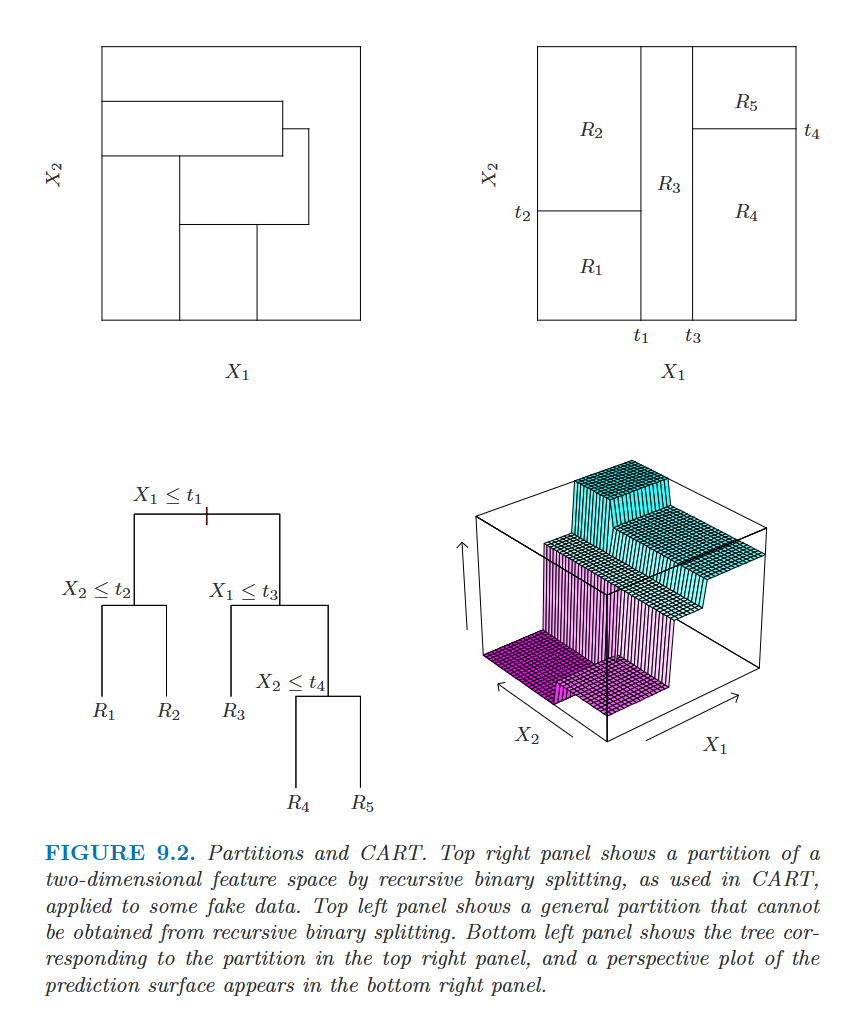
\includegraphics[width=0.95\textwidth]{Chapters/pic/ch_加性模型、树及相关方法/figure_9_2.png}
    \caption{划分与 CART（图 9.2）。右上：对二维特征空间用递归二元划分（CART 采用）得到的分割；左上：无法由递归二元划分得到的一般分割；左下：与右上分割对应的树；右下：预测面的透视图。}
    \label{fig:9_2}
\end{figure}

\textbf{递归二元划分：} 为简化，限制为递归二元划分（图 9.2 右上）。先把空间分成两个区域，用每个区域的 $Y$ 均值建模响应；选择变量和切点使拟合最优。然后其中一个或两个区域再分成两个区域，如此继续直到某个停止规则。例如图 9.2：先在 $X_1 = t_1$ 处分裂，$X_1 \le t_1$ 的区域在 $X_2 = t_2$ 处分裂、$X_1 > t_1$ 的区域在 $X_1 = t_3$ 处分裂，最后 $X_1 > t_3$ 在 $X_2 = t_4$ 处分裂，得到五个区域 $R_1, \ldots, R_5$。对应的回归模型用区域 $R_m$ 中的常数 $c_m$ 预测 $Y$：
\begin{equation}\label{eq:9_9}
    \hat f(X) = \sum_{m=1}^{5} c_m\, I\{(X_1, X_2) \in R_m\}
\end{equation}

同一模型可用二元树表示（图 9.2 左下）：数据集在树顶，满足每个节点条件的观测走左支、否则走右支；终结点（叶）对应区域 $R_1, \ldots, R_5$。右下是预测面的透视图。

\textbf{关键优势：可解释性。} 特征空间划分由单棵树完整描述；两个以上输入时划分难画，但树表示同样工作。这在医学中很流行，因为它模仿医生思考方式——树根据病人特征把总体分层为高/低结果。

\subsection{回归树}

如何生长回归树？数据为 $N$ 个观测 $(x_i, y_i)$，$x_i = (x_{i1}, \ldots, x_{ip})$。算法需自动决定分裂变量、切点、以及树形（topology）。先假设已有 $M$ 个区域 $R_1, \ldots, R_M$，用每个区域的常数 $c_m$ 建模：
\begin{equation}\label{eq:9_10}
    f(x) = \sum_{m=1}^{M} c_m\, I(x \in R_m)
\end{equation}
以最小化平方和 $\sum_i (y_i - f(x_i))^2$ 为准则，最优 $\hat c_m$ 是区域 $R_m$ 中 $y_i$ 的平均：
\begin{equation}\label{eq:9_11}
    \hat c_m = \mathrm{ave}(y_i \mid x_i \in R_m)
\end{equation}

\textbf{贪心算法：} 求最小化平方和的全局最优二元划分通常计算上不可行，因此用贪心算法。从全部数据出发，考虑分裂变量 $j$ 和切点 $s$，定义两个半平面：
\begin{equation}\label{eq:9_12}
    R_1(j,s) = \{X \mid X_j \le s\},\qquad R_2(j,s) = \{X \mid X_j > s\}
\end{equation}
求使下式最小的 $(j, s)$：
\begin{equation}\label{eq:9_13}
    \min_{j,s}\Bigl[\min_{c_1}\sum_{x_i \in R_1(j,s)}(y_i - c_1)^2 + \min_{c_2}\sum_{x_i \in R_2(j,s)}(y_i - c_2)^2\Bigr]
\end{equation}
对任意 $(j,s)$，内层最小化由 $\hat c_1 = \mathrm{ave}(y_i \mid x_i \in R_1(j,s))$、$\hat c_2 = \mathrm{ave}(y_i \mid x_i \in R_2(j,s))$ 解出。对每个分裂变量，切点 $s$ 的确定可很快完成，扫描全部输入即可求最佳 $(j,s)$。找到最佳分裂后，把数据分成两个区域，在每个区域重复分裂过程。

\textbf{树该长多大？} 大树可能过拟合，小树可能漏掉重要结构。树大小是控制复杂度的调节参数，应自适应选择。一种做法是只在分裂使平方和下降超过阈值时才分裂——但这太短视（看似无用的分裂可能带来其下很好的分裂）。\textbf{首选策略：先长一棵大树 $T_0$}，只在达到最小节点大小（如 5）时停止；然后用\textbf{代价复杂度剪枝（cost-complexity pruning）}。

定义子树 $T \subset T_0$ 为对 $T_0$ 剪枝得到的任意树（折叠任意内部节点）。设 $|T|$ 为 $T$ 的终结点数，定义
\begin{equation}\label{eq:9_15}
    N_m = \#\{x_i \in R_m\},\qquad \hat c_m = \frac{1}{N_m}\sum_{x_i \in R_m} y_i,\qquad Q_m(T) = \frac{1}{N_m}\sum_{x_i \in R_m}(y_i - \hat c_m)^2
\end{equation}
代价复杂度准则：
\begin{equation}\label{eq:9_16}
    C_\alpha(T) = \sum_{m=1}^{|T|} N_m Q_m(T) + \alpha |T|
\end{equation}
对每个 $\alpha$，求使 $C_\alpha(T)$ 最小的子树 $T_\alpha \subseteq T_0$。调节参数 $\alpha \ge 0$ 控制树大小与拟合的权衡：$\alpha$ 大 → 树小，$\alpha$ 小 → 树大，$\alpha = 0$ 时解为全树 $T_0$。

对每个 $\alpha$ 存在唯一的最小化 $C_\alpha(T)$ 的最小子树 $T_\alpha$。用\textbf{最弱链接剪枝（weakest link pruning）}求 $T_\alpha$：依次折叠使 $\sum_m N_m Q_m(T)$ 每节点增加最小的内部节点，直到单节点（根）树。这给出有限子树序列，必含 $T_\alpha$。$\alpha$ 用五折或十折交叉验证估计：选使交叉验证平方和最小的 $\hat\alpha$，最终树为 $T_{\hat\alpha}$。

\subsection{分类树}

若目标是取值 $1, \ldots, K$ 的分类结果，树算法的变化只在节点分裂和剪枝准则。回归用平方误差节点不纯度 $Q_m(T)$（式 \eqref{eq:9_15}），不适合分类。在节点 $m$（区域 $R_m$，$N_m$ 个观测）中，设
\[
    \hat p_{mk} = \frac{1}{N_m}\sum_{x_i \in R_m} I(y_i = k)
\]
为节点 $m$ 中类 $k$ 的比例。把节点 $m$ 中的观测分类到多数类 $k(m) = \argmax_k \hat p_{mk}$。节点不纯度 $Q_m(T)$ 的度量包括：
\begin{equation}\label{eq:9_17}
    \begin{aligned}
        \text{误分类误差：} & 1 - \hat p_{mk(m)} \\
        \text{Gini 指数：} & \sum_{k \neq k'} \hat p_{mk}\hat p_{mk'} = \sum_{k=1}^{K}\hat p_{mk}(1 - \hat p_{mk}) \\
        \text{交叉熵（偏差）：} & -\sum_{k=1}^{K}\hat p_{mk}\log\hat p_{mk}
    \end{aligned}
\end{equation}
两类情形（$p$ 为第二类比例）下三者分别为 $1 - \max(p, 1-p)$、$2p(1-p)$、$-p\log p - (1-p)\log(1-p)$（图 9.3）。三者相似，但交叉熵和 Gini 指数\textbf{可微}，更适合数值优化。分裂节点时需用两个子节点的观测数 $N_{mL}, N_{mR}$ 加权不纯度。

此外，交叉熵和 Gini 对节点概率变化比误分类率更敏感。例：两类各 400 观测 $(400,400)$，一个分裂产生 $(300,100)$ 和 $(100,300)$，另一个产生 $(200,400)$ 和 $(200,0)$——两者误分类率都是 0.25，但后者产生\textbf{纯节点}、更可取；Gini 和交叉熵对后者更低。因此生长树时用 Gini 或交叉熵；剪枝时三种都可用，但通常用误分类率。

\textbf{Gini 的两种解释：} ① 不把观测分到多数类，而以概率 $\hat p_{mk}$ 分到类 $k$，则该规则在节点内的期望训练误差率正是 Gini 指数 $\sum_{k\neq k'}\hat p_{mk}\hat p_{mk'}$；② 把每个观测编码为类 $k$ 则 1、否则 0，节点内 0-1 响应的方差为 $\hat p_{mk}(1 - \hat p_{mk})$，对所有类求和即 Gini 指数。

\subsection{其他问题}

\textbf{分类预测变量：} 有 $q$ 个无序取值的预测变量分裂时，有 $2^{q-1} - 1$ 种把 $q$ 个值分成两组的可能划分，$q$ 大时计算不可行。但 0-1 结果时计算可简化：按结果类 1 中的比例排序预测变量类别，然后当作有序预测变量分裂——可证明这在交叉熵或 Gini 意义上给出所有 $2^{q-1}-1$ 种分裂中的最优分裂（定量结果 + 平方损失也成立，按结果均值递增排序；Fisher, 1958）。多类别结果无此简化。\textbf{注意：} 划分算法倾向偏爱水平数 $q$ 多的分类预测变量（选择越多越容易对当前数据找到好的），$q$ 大时会导致严重过拟合，应避免。

\textbf{损失矩阵：} 分类中某些类误分类的后果更严重（如把有心脏病的人预测为没有）。定义 $K \times K$ 损失矩阵 $L$，$L_{kk'}$ 是把类 $k$ 观测分成类 $k'$ 的损失，通常 $L_{kk} = 0$。可把 Gini 指数修改为 $\sum_{k \neq k'} L_{kk'}\hat p_{mk}\hat p_{mk'}$（随机规则的期望损失）——多类有效，但二类时因系数为 $L_{kk'} + L_{k'k}$ 而无效果。二类更好的方法是对类 $k$ 的观测加权 $L_{kk'}$（仅当作为 $k$ 的函数 $L_{kk'}$ 不依赖 $k'$ 时可用于多类）。观测加权可配合偏差使用，效果是改变类的先验概率。终节点中经验贝叶斯规则分类到 $k(m) = \argmin_k \sum_\ell L_{\ell k}\hat p_{m\ell}$。

\textbf{缺失预测值：} 丢弃含缺失值的观测可能严重削减训练集；填充（如均值）也可行。树模型有更好的两种方法：① 分类预测变量：为「缺失」建一个新类别；② 更一般：\textbf{替代变量（surrogate variables）}。分裂时只用该预测变量不缺失的观测；选定最佳（主）预测变量和切点后，形成替代预测变量和切点列表——第一替代是最能模仿主分裂的预测变量，第二替代次之，依次类推。训练或预测中，若主分裂变量缺失，就依次使用替代分裂。替代分裂利用预测变量间的相关性缓解缺失的影响。缺失数据的一般问题见 §9.6。

\textbf{为什么二元分裂？} 多元分裂（一次分多组）会过快碎片化数据，使下一层数据不足。多元分裂可用一系列二元分裂实现，因此后者更可取。

\textbf{其他树构建方法：} 讨论聚焦 CART。另一流行方法是 ID3 及其后续 C4.5、C5.0（Quinlan, 1993）。早期版本限于分类预测变量、自顶向下且不剪枝；C5.0 与 CART 已很相似。C5.0 独有的最重要特性是推导\textbf{规则集}：树长好后，定义终节点的分裂规则有时可简化（去掉一个或多个条件不改变落入节点的观测子集），得到简化的规则集——不再是树结构，但更简单、对用户更有吸引力。

\textbf{线性组合分裂：} 可允许沿 $\sum_j a_j X_j \le s$ 形式的线性组合分裂，权重 $a_j$ 和切点 $s$ 优化以最小化相关准则（如 Gini）。可提高预测力但损害可解释性；切点搜索的离散性使权重无法用光滑优化。更好的方式是在 \textbf{HME（专家分层混合）}模型中引入（§9.5）。

\textbf{树的不稳定性：} 主要问题是高方差。数据的微小变化常导致完全不同的分裂序列，使解释不稳。主因是过程的层次性：顶层分裂的错误会传播到其下所有分裂。可用更稳定的分裂准则缓解，但固有不确定性无法消除——这是从数据估计简单树结构的代价。\textbf{Bagging（§8.7）平均许多树来降低此方差}。

\textbf{缺乏光滑性：} 预测面不光滑（图 9.2 右下）。0/1 损失分类下影响不大（类概率估计的偏差影响有限），但回归设置中会降低性能（通常期望底层函数光滑）。\textbf{MARS}（§9.4）可看作缓解此缺点的 CART 修正。

\textbf{难以捕捉加性结构：} 树难以建模加性结构。例：$Y = c_1 I(X_1 < t_1) + c_2 I(X_2 < t_2) + \varepsilon$。二元树第一层在 $X_1$ 上近 $t_1$ 分裂；下一层需在 $X_2$ 的 $t_2$ 处分裂两个节点才能捕捉加性结构——数据充足时可能发生，但模型没有被特别鼓励去找这种结构。若有十个加性效应，需很多凑巧的分裂才能重建结构。MARS 放弃树结构以捕捉加性结构。

\subsection{spam 例子（续）}

对 spam 数据应用分类树方法：用偏差度量生长树、误分类率剪枝。图 9.4 显示 10 折交叉验证误差率随剪枝树大小的变化（±2 标准误）；注意交叉验证误差由 $\alpha$ 值序列索引（不同折生长的树，同一 $\alpha$ 可能意味着不同大小）。误差在约 17 个终结点处变平（用「1 标准误」规则），得到剪枝树（图 9.5）。树选出的 13 个不同特征中有 11 个与加性模型的 16 个显著特征重叠（表 9.2）。总体误差率（表 9.3，9.3\%）比加性模型（表 9.1，5.3\%）约高 50\%。

看图 9.5 最右分支：若 ch\$ 字符比例超过 5.5\% 则有 spam 警告；但若 hp 短语频繁出现，则更像公司业务、判为 email（22 个满足条件的测试用例全部正确分类）；若第二个条件不满足且 CAPAVE（重复大写字母平均长度）> 2.9，判为 spam（227 个测试用例中仅 7 个误分类）。

医学中常用\textbf{灵敏度（sensitivity）}与\textbf{特异度（specificity）}刻画规则：灵敏度 = 真实有病时预测有病的概率；特异度 = 真实无病时预测无病的概率。把 spam/email 视为有病/无病，由表 9.3 得：
\[
    \text{灵敏度} = 100 \times \frac{33.4}{33.4 + 5.3} = 86.3\%,\qquad
    \text{特异度} = 100 \times \frac{57.3}{57.3 + 4.0} = 93.4\%
\]

\textbf{ROC 曲线：} 通过改变损失 $L_{01}, L_{10}$ 的相对大小可提高灵敏度/降低特异度（或反之）。本例要避免把好 email 标为 spam，故希望特异度很高——设 $L_{01} > 1$、$L_{10} = 1$ 实现。\textbf{ROC 曲线}是评估灵敏度与特异度权衡的常用总结：随分类规则参数变化，绘制灵敏度对特异度的曲线。对 17 节点树在 $L_{01}$ 从 0.1 到 10 变化下应用贝叶斯规则，得到图 9.6 的 ROC 曲线；\textbf{曲线下面积（AUC）}约 0.95。GAM 模型（§9.1.2）的 ROC 曲线对任何损失都更好，AUC 0.98。用损失 $L_{01} = 5, L_{10} = 1$ 生长同大小树（观测加权），在高特异度处灵敏度更高——对这个应用明显优于原树。

\textbf{c 统计量：} AUC 有时称为 c 统计量。可证 AUC 等价于 \textbf{Mann--Whitney U 统计量}（或 Wilcoxon 秩和检验）关于两组预测分数中位数差异（Hanley and McNeil, 1982）。评估给标准模型增加一个预测变量的贡献时，c 统计量可能不是有信息量的度量：新预测变量在模型偏差变化上可能非常显著，但 c 统计量只增一点（如去掉显著的 george 项，c 统计量下降不到 0.01）。应检查新预测变量如何在单个样本基础上改变分类（Cook, 2007）。

% ============ §9.3 PRIM：Bump Hunting（引入） ============
\section{PRIM：Bump Hunting（引入）}

基于树的方法（回归）把特征空间划分为盒状区域，使每个盒内响应均值尽可能不同。§9.3 将介绍另一种互补方法 \textbf{PRIM（患者规则归纳法，Patient Rule Induction Method）}，用于寻找特征空间中响应均值特别高的区域——「bump hunting（隆起搜寻）」。其细节将在后续阅读中补充。
